%Making this a subsection because it's still about practicing the models...
\subsection{Thermal and Bond Energy Systems}
\label{act1.2.2}

\begin{fnt}
	\label{fnt1.2.1-1}

Consider again the phenomenon of two substances at different temperatures exchanging energy as they come to thermal equilibrium: \emph{Substance A} and \emph{Substance B}, at initially different temperatures, are placed in contact. They are able to exchange energy as heat, and they can only exchange it with each other. Substance A has a greater initial temperature than Substance B. No phase changes occur during this process.

Use the \EnergyInteractionModel{} to create a logical explanation that unequivocally shows that the following statement about the heat exchange described above for Substances A and B is true or that it is false:

\begin{quote}
	``The energy that is transferred as heat to or from the object with the larger heat capacity must be greater than the energy that is transferred as heat to or from the object with the smaller heat capacity.''
\end{quote}
\end{fnt}

\note{Timing: \unit[\textless3]{min}}{
	\begin{itemize}
		\item The answer may be obvious, but make them explain how they know in the WC discussion. For example, ``With only two energy systems, the magnitude of energy leaving the one must be the same as the magnitude of energy into the second.'' As always, it is important for them to put things into their own words. 
		\item Follow-up question: Ask them what the effect of the different heat capacities will be.
	\end{itemize}
}

\noindent Discuss this FNT in your group and be prepared to explain in the whole class discussion. You do not need to put anything on the board.

\WCD

\begin{fnt}
	\label{fnt1.2.1-2}

Consider the following example of two substances at different temperatures exchanging heat as they come to thermal equilibrium.

A \unit[3.50]{kg} piece of lead and a \unit[1.5]{kg} piece of aluminum, at different temperatures, are placed in contact. They are able to exchange energy as heat and they can only exchange it with each other. The initial temperature of the lead is \unit[48]{\textdegree C}, and the initial temperature of the aluminum is \unit[35]{\textdegree C}. The table on page 5 the course notes has phase change temperatures and values of specific heats for these substances. 

\begin{enumerate}[(a)]
	\item If it is possible (How do you know this?), construct a single, closed \EnergyDiagram{} for the process of lead and aluminum coming to thermal equilibrium.

	\item Write an algebraic expression of energy conservation in terms of the $\Delta E$s of the two energy systems, and then substitute in the appropriate expressions for the $\Delta E$s.

	\item Substitute in all known numerical values. How many unknowns are there in your equation expressing energy conservation?

	\item At an {\em intermediate} point in the entire process described above the lead has reached a temperature of \unit[43]{\textdegree C}.
	
	Follow the instructions for part (a) for the interval that \emph{ends when the lead is at a temperature of \unit[43]{\textdegree C}}. What feature related to the process connects the final temperatures of lead and aluminum that appear in your diagram to each other?

\end{enumerate}
\end{fnt}

\note{Timing: \unit[$\sim$15]{min}}{
	\subsubsection*{What is the purpose of Handout 1.2.2?  (distributed to students)}
	\begin{itemize}
		\item Save time in today's DL. None of the diagrams in the handout needs to be put on the board by students or instructors. 
		\item Everyone has uniform conventions for \EnergyDiagrams{}. 
		\item Illustrates what is appropriate to put on the board for WC discussion. 
		\begin{itemize}
			\item It is not useful to show the algebraic manipulations necessary to get the final answer on the board. Make it clear that in the future, only what is shown in this diagram is what they should put on the board for the WC discussion.
			\item Discourage the students from working out the algebra in class. We want them to understand the difference between ``the physics'', which is illustrated in the diagrams on the handout, and ``the algebra''.
		\end{itemize}
	\end{itemize}
}


\begin{enumerate}[1.]
	\item A student constructed the following \EnergyDiagram{} for Part (a) of \hyperref[fnt1.2.1-2]{this FNT}:

	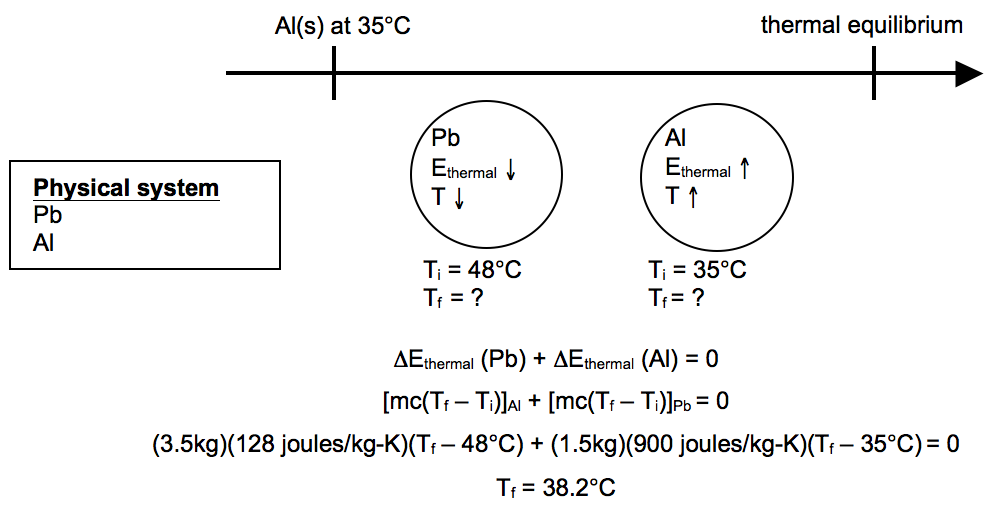
\includegraphics[width=0.7\linewidth]{handout-fnt121-2a}
	
	Discuss the diagram briefly in your group, and identify any questions you have. You don't need to put anything on the board.\footnote{Incidentally, this diagram illustrates how much algebra is useful to put down for the purpose of clear communication in whole class discussions. In general, it is not useful to show the details of solving the algebra on the board. Being able to construct the correct diagram and getting the first three lines of algebra (including verifying the signs of the terms in the third line) are worth most of the credit on an exam.}
	
	\note{}{
		Students inspect diagram for part (a) on the handout and identify any questions. Not necessary to put anything on the board.
		
		If they have questions about the diagram you can respond either to the SG individually, or if you think others might benefit, with the WC. 
	}
	
	\item Put a complete \EnergyDiagram{} on the board for the shorter interval described in Part (d) of \hyperref[fnt1.2.1-2]{this FNT}. What specifically is happening in the process that ``connects'' the two final temperatures (of lead and aluminum) in your diagram? Illustrate this on the board with two separate \TempGraphs{}, one for each substance.
	
	\note{}{
		Put a complete \EnergyDiagram{} on the board for the {\em shorter} interval described in part (d). What is the connection between the two final temperatures in your diagram? 
		\begin{itemize}
			\item The \EnergyDiagram{} is shown directly below.
			\item The connection: the two indicators are correlated with the end of the interval, i.e., they have those values at the same time. This may seem obvious to the point of being trivial, but as the number of terms in the equation expressing energy conservation increases, students have more difficulty seeing the relationship among the various initial and final values.
		\end{itemize}
	}
	
	\note{}{
		\noindent
		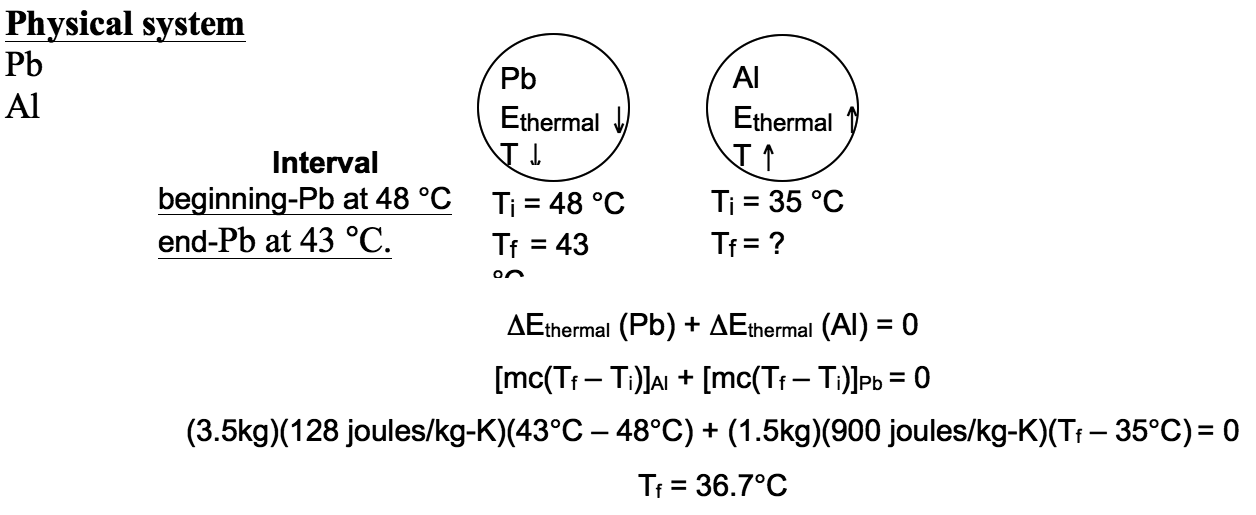
\includegraphics[width=\linewidth]{fnt121-2b}
	}

\WCD 

\end{enumerate}

\begin{fnt}
	\label{fnt1.2.1-3}

Suppose you used a hot pot to convert a \unit[150]{g} piece of ice that was initially at \unit[-15]{\textdegree C} into liquid water at \unit[50]{\textdegree C}.

\begin{enumerate}[(a)]
	\item Represent this process in two complete \EnergyDiagrams{}, one covering the interval from \unit[-15]{\textdegree C} to \unit[0]{\textdegree C} liquid, and the second covering the interval from \unit[0]{\textdegree C} liquid to \unit[50]{\textdegree C}.
	\item Now represent the entire process in one complete \EnergyDiagram{} covering the entire interval.
	\item If your hot pot has a power rating of \unit[600]{watts}, show how to find how long it will take to complete the process. (Make sure you are comfortable using standard units of energy, and that you understand the relation of power to energy.)
\end{enumerate}
\end{fnt}

\note{Timing: \unit[\about10]{min}}{
	
}

\begin{enumerate}[1.]

	\item Again, we consider a student's response to \hyperref[fnt1.2.1-3]{this FNT}. Discuss the diagrams for Part (a) below and identify any questions you have. As before, you don't have to put anything on the board for this part.
	
		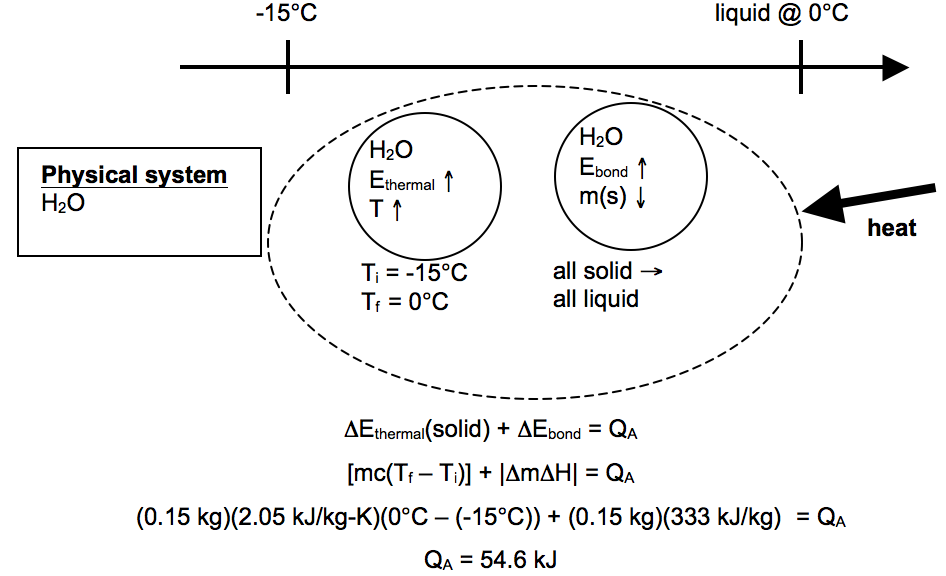
\includegraphics[width=0.55\linewidth]{handout-fnt121-3a1}
		\;
		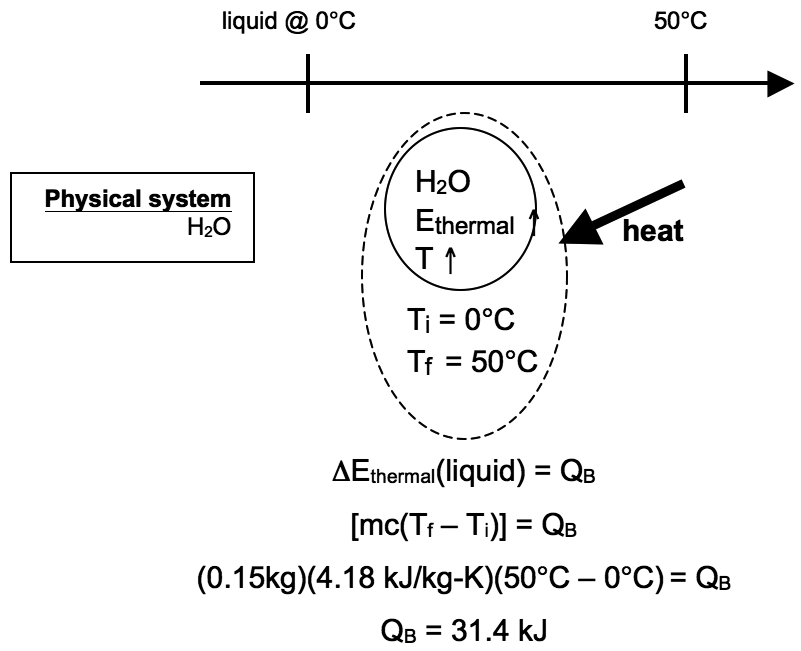
\includegraphics[width=0.35\linewidth]{handout-fnt121-3a2}
	
	\item A student objects to the diagram for Part (b) of \hyperref[fnt1.2.1-3]{this FNT} below because some of the indicators do not correspond to the beginning and end of the overall interval.
	
		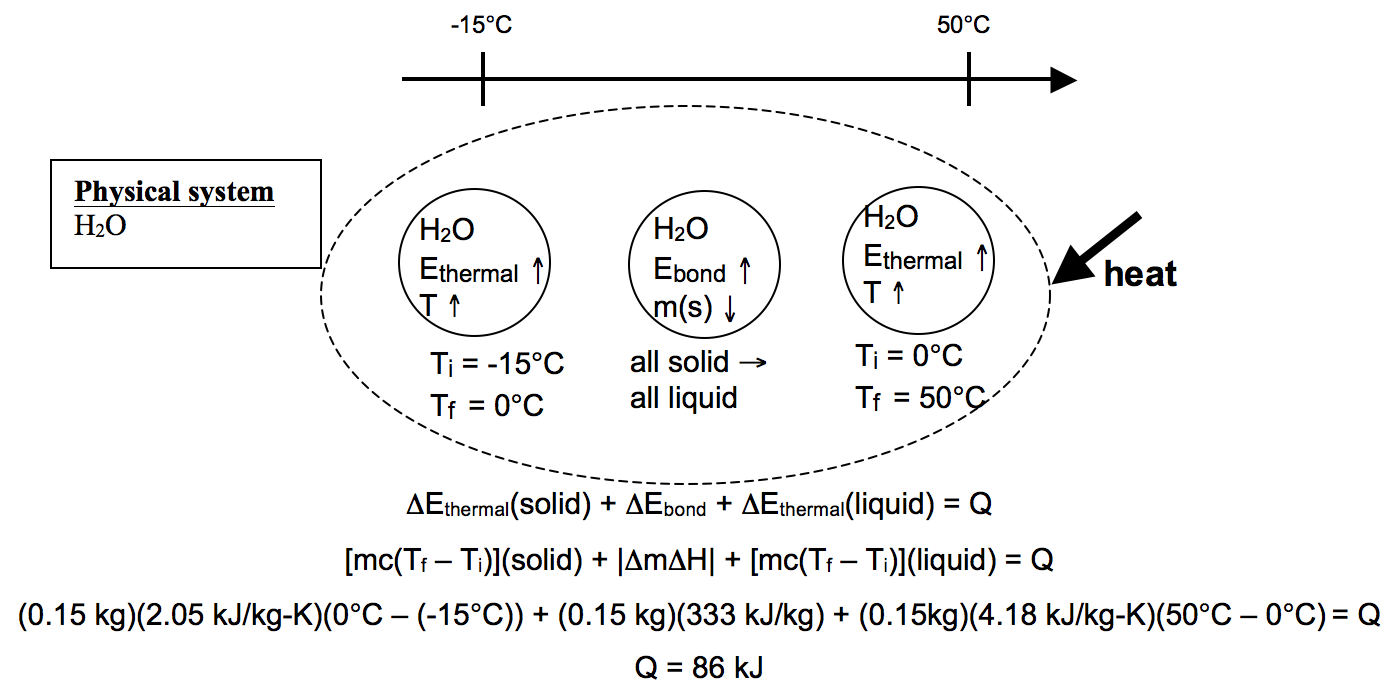
\includegraphics[width=0.7\linewidth]{handout-fnt121-3b}
		
		Another student says that's ok because each physical process in the interval happens sequentially and nothing has been left out. Come to a consensus about which of these two students you agree with and put a brief explanation on the board.
	
	\item Discuss the question about power in Part (c) in your group and identify any questions you have. Make sure you have a clear understanding of the relationship of power to energy. You don't have to put anything on the board for Part (c), but be ready to explain the difference between energy and power if called upon in the whole class discussion.

\WCD

\end{enumerate}

\subsection{Asking Questions and Determining Intervals of Interest}
\label{act1.2.2D}

\begin{fnt}
	\label{fnt1.2.1-4}

\ref{fnt1.2.1-2} and \ref{fnt1.2.1-3} emphasized the significance of the beginning and end of the interval -- we've called them ``initial'' and ``final'' states so far. This FNT illustrates
\begin{enumerate}[(i)]

	\item that the question you're asking determines the interval being analyzed with the \EnergyInteractionModel{}; and

	\item that sometimes it's necessary to adjust the size of the interval in order to be able to use the model.

\end{enumerate}

\noindent The physical process we want to analyze with the \ThreePhaseModel{} and the \EnergyInteractionModel{} is the following:\\

\noindent Imagine you are using your hot pot to gradually add heat to a \unit[500]{g} block of ice that has just been removed from a freezer with an internal temperature of \unit[-25]{\textdegree C}. The hot pot is fairly well insulated, so it is reasonable to assume that all of the heat put into the pot from the electrical heater located in the bottom of the pot goes into the \ce{H2O}. We can also assume that the heat capacity of the pot is much smaller than the heat capacity of \unit[500]{g} of \ce{H2O} (whether solid or liquid), so we can ignore the thermal energy system of the pot itself.

One question we could ask is, ``What is the final state of the water (phase and temperature) after the addition of \unit[252]{kJ} of heat?'' 

\begin{enumerate}[(a)]

	\item Explain why -- based {\em only} on the given information and without further analysis or calculation -- it is \textbf{\em not possible} to construct a {\em single} \EnergyDiagram{} that could be used to determine the final state of the water.
	
		[Hint: try to construct such a diagram. Another way to think about this is whether you can define the final state so that it depends on only one variable without making unjustified assumptions?]

	\item In cases like this, you must first use the model to analyze a {\em shorter interval}. Can you construct an \EnergyDiagram{} that could be used to determine how much energy is needed to increase the temperature of the ice to \unit[0]{\textdegree C}?
	
		Now explain in a few sentences how to proceed using the \EnergyInteractionModel{} to find the final state of the \ce{H2O}.

\end{enumerate}
\end{fnt}

\note{Timing: \unit[\about10]{min}}{
	
}

\begin{enumerate}[1.]

	\item Why is it \emph{not} possible to apply the \textbf{\EnergyInteractionModel{}} in a {\em straightforward} way to the interval of interest -- the interval that ends when all of the \unit[252]{kJ} has been added to the water? In other words, why can't the overall interval be diagrammed using {\em only} the given information prior to doing any further analysis?   Draw a \TempGraph{} to help you make sense of this and to use to explain it. In particular, be sure to make explicit which part of the graph in the diagram refers to which ``energy bubble'' on the \EnergyDiagram{}. [To save time, explanations on the board can be more abbreviated than they would be on an exam. In this case, anything that is unclear can be easily clarified in the whole class discussion.]
	
	\item Explain how to use the \textbf{\EnergyInteractionModel{}} to analyze shorter intervals in order to determine the final state (phase and temperature) of the water.  (Note: ``water,'' without a modifier, usually means \ce{H2O} in any one of its three phases.) Use a \TempGraph{} in your analysis and to use in your explanation.

\WCD 

\end{enumerate}